\section{Descrizione generale}

Le principali fonti di informazione relative all'azienda ospitante derivano dalla consultazione del \emph{sito web} aziendale, effettuata durante la fase di scelta dello stage, 
e dalle interazioni con il tutor aziendale e i membri del team nelle prime fasi conoscitive. Poiché la mia postazione era nella stessa stanza del team nei giorni di presenza in azienda, 
ho inoltre raccolto informazioni di tipo informale osservando il lavoro quotidiano e ascoltando le conversazioni del gruppo. Le informazioni non sono state tutte disponibili prima dell'inizio del progetto, 
ma si sono accumulate gradualmente durante l'intero periodo di stage.

Halue S.r.l. è una società benefit di consulenza tecnica orientata all'adozione di soluzioni basate sull'intelligenza artificiale e alla fornitura di servizi 
sia \emph{B2C} (business-to-consumer) sia \emph{B2B} (business-to-business). 
Le attività dell'azienda si articolano in diversi servizi, tra cui: progettazione e gestione di soluzioni per l'\emph{e-commerce} (commercio elettronico), 
implementazione di sistemi di gestione delle relazioni con i clienti (\emph{CRM}, Customer Relationship Management), 
servizi legati all'IA (ad es. sviluppo di agenti intelligenti) e percorsi di formazione rivolti ai clienti.

\medskip
\noindent\textbf{Contesto organizzativo}

Le informazioni relative al contesto organizzativo derivano sia dalle discussioni con il tutor aziendale sull'andamento del progetto, 
sia dalle conversazioni con altri membri del team. L'organizzazione concilia modalità di lavoro ibride e in \emph{full remote}. 
Il team tiene \emph{stand-up meeting} quotidiani per allinearsi sul lavoro svolto nella giornata precedente e sugli obiettivi della giornata corrente; 
periodicamente vengono organizzati incontri informali per mantenere buoni rapporti fra i membri e rinsaldare i valori aziendali.

La comunicazione interna si sviluppa su più livelli, con strumenti scelti in funzione delle esigenze organizzative:

\begin{itemize}
\item richieste di aiuto di carattere informale vengono spesso rivolte verbalmente; richieste più dettagliate o tecniche vengono inserite nello strumento di gestione dei progetti, dove ogni membro può \emph{postare} dubbi o proposte all'interno del proprio ramo di lavoro;
\item richieste di \emph{meeting} o chiarimenti che richiedono l'accordo su un orario sono gestite tramite la piattaforma di messaggistica condivisa dal team;
\item infine, le comunicazioni di natura amministrativa o burocratica vengono inviate tramite Gmail.
\end{itemize}

\medskip
\noindent\textbf{Contesto produttivo}

Le informazioni sul contesto produttivo provengono dalle interazioni con il tutor e dai colloqui con i colleghi. 
Dal punto di vista produttivo, l'azienda privilegia il rapido ingresso delle soluzioni nel mercato, adottando architetture che riducano gli ostacoli al 
\emph{deployment} (messa in distribuzione del software in ambiente operativo). Ho riscontrato l'uso dell'approccio \emph{Agile} (metodologie iterative e incrementali per adattarsi rapidamente ai cambiamenti dei requisiti) 
con gestione tramite \emph{backlog} (elenco prioritizzato di attività) e strumenti di tracciamento. La comunicazione interna è adattata alle necessità operative.

\begin{figure}[htbp]
    \centering
    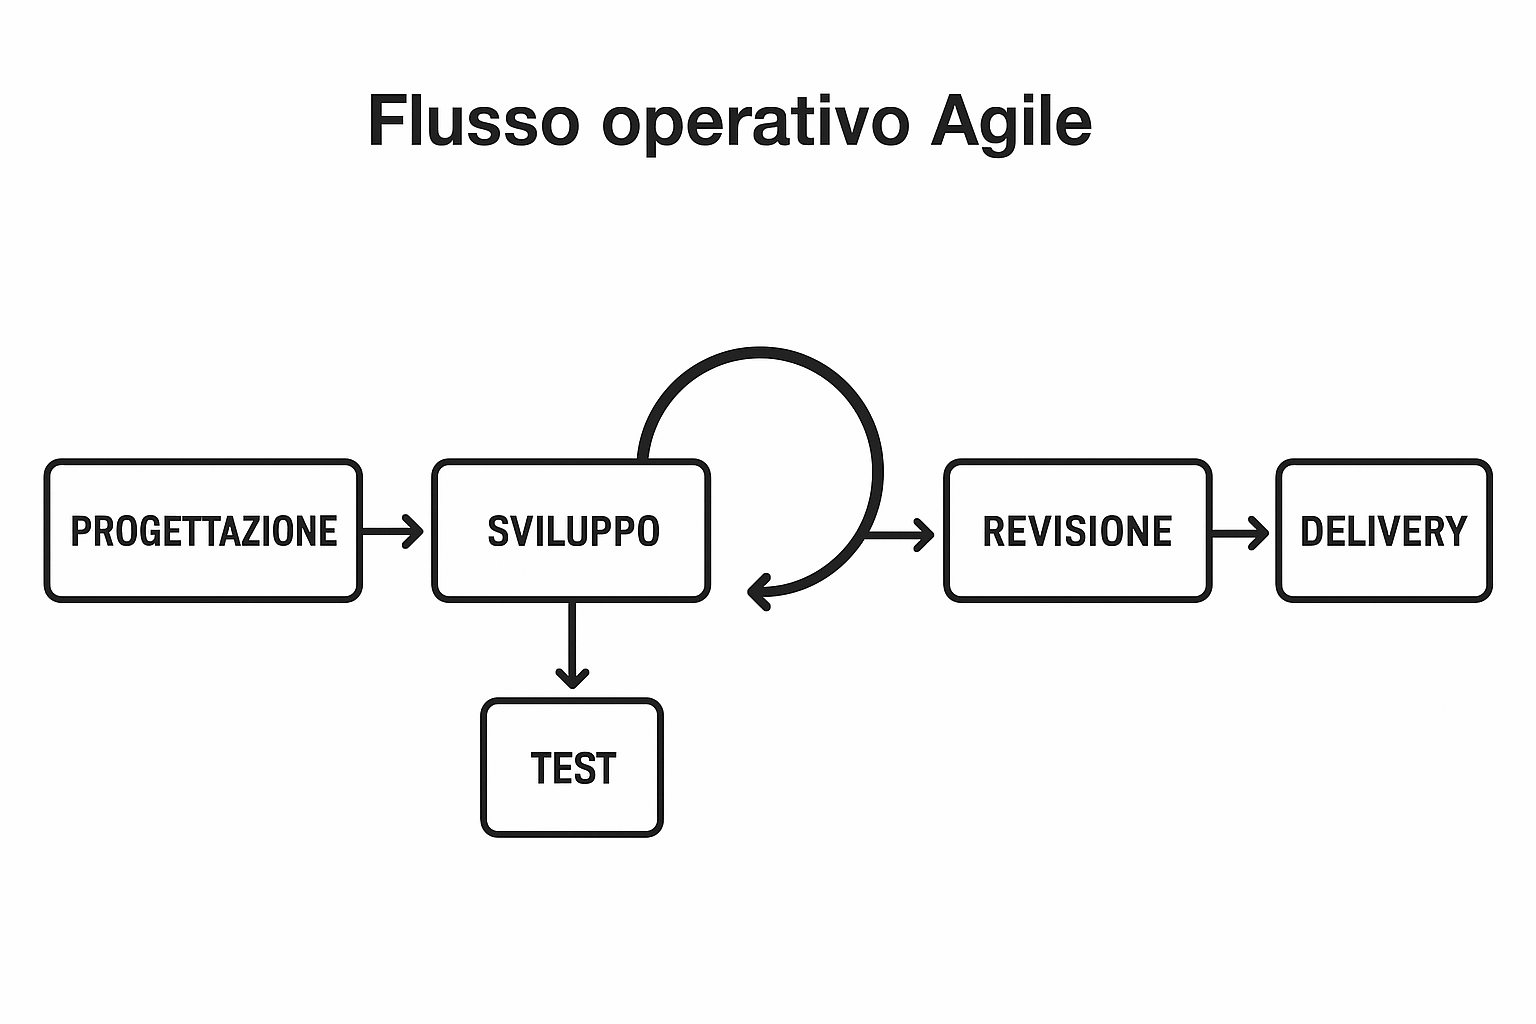
\includegraphics[width=0.8\textwidth]{azienda/metodo_agile}
    \caption{Flusso operativo Agile.}
    \label{fig:agile}
\end{figure}

Sono presenti ambienti separati per il \emph{testing} (collaudo) e per la produzione, oltre a procedure di rilascio automatizzate predisposte per i singoli progetti. 
Si alternano attività di \emph{delivery} (consegna/erogazione del servizio) su progetti custom e attività di supporto e manutenzione post-consegna.

\medskip
\noindent\textbf{Clientela}

Le informazioni sulla clientela derivano dall'analisi del sito web aziendale condotta nella fase di scelta dello stage e dall'osservazione dei progetti a cui ho partecipato. 
La clientela va dalle piccole e medie imprese con esigenze di commercio elettronico fino a grandi committenti che richiedono integrazioni complesse e soluzioni \emph{CRM} articolate. 
Sono presenti commesse nel settore privato (retail, distributori, operatori \emph{B2B}) e interventi rivolti a processi interni di organizzazioni di maggiori dimensioni.

\medskip
\noindent\textbf{Propensione all'innovazione}

La propensione all'innovazione dell'azienda è emersa chiaramente dall'analisi del progetto a me assegnato e dal modo in cui esso si è integrato nel contesto produttivo. 
Questa inclinazione si manifesta attraverso un'attenzione costante alla formazione interna, l'adozione di architetture e pratiche tecnologiche moderne e la sperimentazione su 
iniziative legate all'intelligenza artificiale. Al contempo, l'approccio rimane pragmatico: quando i vincoli operativi, i requisiti di affidabilità o i tempi di consegna lo richiedono, 
l'azienda privilegia soluzioni consolidate per garantire stabilità e robustezza.

Ho osservato una chiara divisione tra attività orientate allo sviluppo operativo e attività focalizzate sulla ricerca e sperimentazione. 
L'attività di ricerca comprende indagini tecniche per valutare nuove tecnologie e framework, lo sviluppo di \emph{proof-of-concept} (\emph{PoC}: prototipo sperimentale) e 
prototipi per dimostrare la fattibilità di idee innovative, sperimentazioni comparative e benchmark per valutare prestazioni, scalabilità e costi, oltre alla preparazione di dimostrazioni e 
documentazione tecnica da sottoporre a \emph{stakeholder} (persona o gruppo che ha interesse e influenza attività e decisioni di un'organizzazione o di un progetto).

La parte del team dedita alla ricerca crea e mette a disposizione ambienti di sperimentazione controllato con 
branch sperimentali nel sistema di controllo versione e procedure formali per la validazione dei PoC prima di un eventuale inserimento in produzione. 

Nel complesso, la propensione all'innovazione risulta essere sia presente che ben strutturata: l'azienda favorisce l'emergere di nuove soluzioni e competenze mantenendo al contempo processi e controlli tecnici volti a 
garantire la qualità e la stabilità dei prodotti e dei servizi offerti.